\documentclass[a4paper,12pt]{article}
\usepackage{amsmath,amsfonts,amssymb} % Math packages
\usepackage{mathtools} % For defining floor and ceiling functions
\usepackage{comment}
\usepackage{amsthm}    % Theorems
\usepackage{bm}        % Bold math
\usepackage{bbm}       % More bold math?
\usepackage{array}     % Better tables
\usepackage{physics}   % derivatives and partials
\usepackage{float}     % Better positioning [H]
\usepackage{framed}    % Framed boxes
\usepackage{geometry}  % Required for adjusting page dimensions and margins
\usepackage{graphicx}  % Include images
\usepackage{multirow}  % multicolumn tables
\usepackage{pgfplots}  % Create plots in latex
\usepackage{siunitx}   % SI unit system
\usepackage{listings}  % Code environments
\usepackage[shortlabels]{enumitem} %lets us change the enumeration to (a), (b), ...
\usepackage{booktabs}  % Better looking horizontal rules
\usepackage{makecell}  % Pre-formatting of column heads
\usepackage{hyperref}  % Clickable links
\usepackage{tikz}      % Graphs
\usepackage{cancel}    % Cancel out terms
\usetikzlibrary{shapes,arrows,positioning} % Graph arrows
\usetikzlibrary{automata,positioning,fit,shapes.geometric,backgrounds} % Node grouping
\usetikzlibrary{calc, tikzmark}  % Marking equations
\usepackage{subcaption}
\usepackage{wrapfig}
\renewcommand{\arraystretch}{1.6}

\usepackage{mathtools}
\newcommand{\defeq}{\vcentcolon=}
\newcommand{\eqdef}{=\vcentcolon}

\newtheorem{theorem}{Theorem}[section]
\newtheorem{definition}{Definition}[section]
\newtheorem{lemma}{Lemma}[section]
\newtheorem{assumption}{Assumption}[section]
\theoremstyle{definition}
\newtheorem{question}{Question}
\pgfplotsset{width=10cm,compat=1.9}

% stats commands
\newcommand{\E}{\mathbb{E}}
\newcommand{\Var}{\mathbb{V}\mathrm{ar}}
\newcommand{\Cov}{\mathbb{C}\mathrm{ov}}
\newcommand{\Risk}{\mathcal{R}}
\newcommand{\Bias}{\mathrm{Bias}}
\newcommand{\MSE}{\mathrm{MSE}}
\newcommand{\Normal}{\mathcal{N}}
\newcommand{\Exponential}{\mathrm{Exp}}
\newcommand{\Poisson}{\mathrm{Poisson}}
\newcommand{\Bernoulli}{\mathrm{Bernoulli}}
\newcommand{\Binomial}{\mathrm{Binomial}}
\newcommand{\Uniform}{\mathrm{Uniform}}
\newcommand{\Beta}{\mathrm{Beta}}
\newcommand{\GammaDist}{\mathrm{Gamma}}
\DeclareMathOperator*{\argmax}{arg\,max}
\DeclareMathOperator*{\argmin}{arg\,min}

% Common number sets
\newcommand{\N}{\mathbb{N}}
\newcommand{\R}{\mathbb{R}}
\newcommand{\Q}{\mathbb{Q}}
\newcommand{\Z}{\mathbb{Z}}
\newcommand{\C}{\mathbb{C}}

% Cs stuff
\newcommand{\bigO}{\mathcal{O}}

% Indicator function
\newcommand{\Ind}[1]{\mathbbm{1}_{\{#1\}}}

\DeclarePairedDelimiter\ceil{\lceil}{\rceil}
\DeclarePairedDelimiter\floor{\lfloor}{\rfloor}
\DeclarePairedDelimiter\angleb{\langle}{\rangle}

\geometry{
  paper=a4paper, % Paper size, change to letterpaper for US letter size
  margin=1in, % Margin size
  headheight=14pt, % Header height
  footskip=1.5cm, % Space from the bottom margin to the baseline of the footer
  headsep=1.2cm, % Space from the top margin to the baseline of the header
}

\makeatletter
\renewcommand{\maketitle}{
  \begin{center}
    {\large\bfseries \@title \par}
    \vskip 1em
    {\@author}
  \end{center}
}
\makeatother


% The title of the report
\title{Efficient Global Content Recovery for Multi-View Data}
% Write your name in author
\author{Ryan Jackson, David Zhao, Dowoo Kim}

\begin{document}

\maketitle

\section{Introduction and Motivation}
Multi-view representation learning aims to recover shared causal variables (``content") while discarding view-specific noise (``style"). While recent work by Yao et al. \cite{yao2024multiviewcausalrepresentationlearning} provides theoretical guarantees for \textit{block-identifiability} using a masking mechanism, their framework faces three practical limitations:

\begin{wrapfigure}[12]{r}{0.35\textwidth}
  \centering
  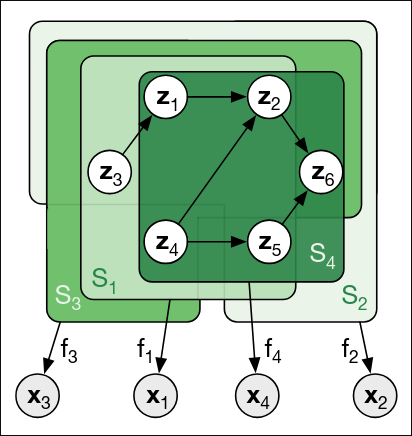
\includegraphics[width=0.25\textwidth]{figures/yao_multiview.png}
  \caption{\small{Multi-view setup under partial observability \cite{yao2024multiviewcausalrepresentationlearning}.} Directed arrows between latents indicate causal relations}
  \label{fig:setup}
\end{wrapfigure}

\begin{enumerate}[noitemsep, topsep=0pt]
  \item \textbf{Complexity:} simultaneously evaluating all possible view subsets is unscalable.
  \item \textbf{Assumptions:} relies on known, fixed view-specific latent dimensions.
  \item \textbf{Optimization:} uses a non-convex $L_{0}$ penalty that is difficult to optimize.
\end{enumerate}

In Section \ref{sec:method}, we propose an efficient alternative for \textit{global content recovery}. Our approach offers three key contributions: (i) we eliminate combinatorial overhead by focusing on the intersection of all views; (ii) we relax dimensionality constraints by requiring only an \textit{overestimation} of the content dimension; and (iii) we utilize the differentiable \textit{hard concrete distribution} \cite{louizos2018learningsparseneuralnetworks} to enable stable, end-to-end mask optimization. This provides a more scalable and robust framework for real-world causal representation.

\section{Problem Setup and Notation} \label{sec:theory}
We formalize the environment by assuming the existence of (possibly causally dependent) ground-truth latent variables $\mathbf{z} = (\mathbf{z}_1, \dots, \mathbf{z}_N) \sim p_{\mathbf{z}}$ taking values in $\mathcal{Z} \subseteq \mathbb{R}^N$. Instead of observing $\mathbf{z}$ directly, we have access to a set of $K$ distinct views, denoted as $\mathbf{x} = (\mathbf{x}_1, \dots, \mathbf{x}_K)$. Crucially, each view $\mathbf{x}_k$ is only a partial observation of the environment, generated by a specific subset of the latent variables, $\mathbf{z}_{S_k}$, where the indices are defined by a subset $S_k \subseteq [N]=\{1, \dots, N\}$. For each view, there is an associated observation space $\mathcal{X}_k$, and a smooth and invertible mixing function $f_k : \mathcal{Z}_{S_{k}} \to \mathcal{X}_{k}$, so that $\mathbf{x}_k = f_k(\mathbf{z}_{S_k})$. See Fig. \ref{fig:setup} for an illustration of the setup.

Our objective is to recover the \textit{global content} $\mathbf{z}_C$ — the latent variables shared across \textit{all} views ($C = \bigcap_{k=1}^K S_k$). We prioritize these variables as they represent the core causal factors that are invariant across different observations, which are essential for tasks like generalization and transfer learning. The remaining view-specific latents $\mathbf{z}_{S_k \setminus C}$ are considered \textit{style} variables, which may contain noise or irrelevant information specific to each view.

We aim for \textit{block-identifiability}, meaning our learned representations $\hat{\mathbf{c}}$ should recover the block of true content variables up to a smooth bijection. Importantly, this definition departs from the stricter notion of \textit{identifiability}, which requires recovering each individual latent variable up to some trivial transformation.

As a last bit of notation, we use a selection operator $\oslash$ to apply masking. Formal definitions of block-identifiability and the selection operator are provided in Appendix \ref{app:definitions}.

\section{Theoretical Background} \label{sec:Theory}
Our work builds on the theoretical foundation established by Yao et al. \cite{yao2024multiviewcausalrepresentationlearning}, who provided two primary guarantees for multi-view causal representation learning. Their initial result proves that for any fixed subset of two or more views, shared content is block-identifiable via \textit{content encoders} $g_k$ by minimizing an objective comprising an alignment term (contrastive loss in Euclidean geometry) and a differential entropy regularizer (to prevent collapse)

To avoid the computational burden of retraining encoders for every possible subset of views, their subsequent result introduces learned \textit{content selectors} (masks) and \textit{projections}. This architecture achieves simultaneous block-identifiability of the shared content of any subset of two or more views using shared \textit{view-specific encoders}. An information-sharing regularizer (sparsity penalty) prevents the model from trivially labeling all dimensions as ``shared", forcing a clean separation between invariant content and view-specific style. We leave further intuitions and detailed explanations of the theoretical results to Appendix \ref{app:theory}.

While the latter result may be theoretically robust, this framework presents significant practical challenges: it assumes that the number of view-specific latent dimensions $|S_k|$ is known a priori, and requires a combinatorial alignment process over all possible subsets of views, which is computationally infeasible as the number of views increases. We address these bottlenecks in Section \ref{sec:method} by narrowing our scope to \textit{global} content recovery, and by relaxing these restrictive dimensionality constraints.

\section{Method}
\label{sec:method}
We focus on recovering the global shared content $\mathbf{z}_C$ by aligning representations across all $K$ views. Additionally, unlike previous theoretical frameworks that require the number of content dimensions $|C|$ or view-specific latent dimensions $|S_{k}|$ to be known, we operate under a relaxed setting where all view-specific encoders $\{ r_k \}_{k=1}^{K}$ map to a shared latent space of dimension $d$. We assume only that this common dimension $d$ is an \textit{overestimation} of the true content dimension (i.e., $d \ge |C|$).

To bridge the gap between theory and practice, we introduce two primary modifications. First, we implement a \textit{shared masking mechanism} where a single binary mask $\mathbf{\phi} \in \{0, 1\}^d$ is applied globally across the outputs of all encoders $\{r_k\}_{k=1}^K$. This enforces a common latent subspace for shared content and significantly simplifies the per-view selectors required by Theorem \ref{thm:allContBlocks}. We optimize this mask end-to-end using a \textit{hard concrete distribution} \cite{louizos2018learningsparseneuralnetworks}, which provides a differentiable surrogate for $L_0$ regularization, while potentially learning exact binary values to prune unshared dimensions.

Second, we replace the loss in the theoretical objective involving intractable differential entropy terms with a \textit{Symmetric InfoNCE} loss \cite{oord2019representationlearningcontrastivepredictive, radford2021learning}. This self-supervised surrogate enforces alignment through pairwise contrast across all views while preventing dimensional collapse by maximizing a lower bound on mutual information. The total objective is defined as
\begin{equation*}
  \mathcal{L}_{\text{total}} = \mathcal{L}_{\text{SymInfoNCE}} + \lambda \text{Reg}(\phi),
\end{equation*}
where $\mathrm{Reg}(\phi)$ is the differentiable sparsity regularizer on the mask and $\lambda$ is a hyperparameter controlling the strength of the regularization. Detailed formulations of the masking distribution and the contrastive objective are provided in Appendix \ref{app:approach_details}.

\section{Experiments}

Our experiments follow the same flavor as in \cite{daunhawer2023identifiabilityresultsmultimodalcontrastive} and \cite{yao2024multiviewcausalrepresentationlearning}: we first evaluate the performance of our method on synthetic data, where we have access to the ground truth latent variables. Then, we apply our method to the \textit{Multimodal3DIdent} dataset \cite{daunhawer2023identifiabilityresultsmultimodalcontrastive}, which consists of blender-rendered images of 3D objects, paired with descriptive text captions.
The code is available in our Github repository\footnote{\url{https://github.com/Virusmint/multiview-sparse}} and builds upon the code of Daunhawer et al. \cite{daunhawer2023identifiabilityresultsmultimodalcontrastive} and Yao et al. \cite{yao2024multiviewcausalrepresentationlearning}.

To evaluate block-identifiability, we quantify the information captured in learned representations by predicting ground-truth latents from embeddings. Successful recovery is defined by high predictive performance for shared content and near-chance performance for style factors (absent statistical dependencies). We report the $R^2$ scores from linear regression for continuous latent factors and the classification accuracy from logistic regression for discrete factors.

\subsection{Numerical Experiment}

We generate synthetic data in which 10 \textit{independent} latent variables are sampled from a Gaussian distribution $\mathbf{z} \sim \Normal(0, \mathbf{I}_\mathbf{z})$. Furthermore, we create 8 views from the latent variables, with each view $\mathbf{x}_k$ generated by an invertible nonlinear transformation of a subset $S_k$ of the latent variables: $\mathbf{x}_k = f_k(\mathbf{z}_{S_{k}})$. Importantly, only 2 latents, $\mathbf{z}_1$ and $\mathbf{z}_2$, are shared (content) across all views, while the remaining latents are view-specific. We summarize our results in Fig. \ref{fig:num_exp_indep} and defer the implementation details to Tab. \ref{tab:hyperparams_num}.

We also defer the results of an additional experiment to Appendix \ref{app:AdditonalExpResults}, where \textit{causal} dependencies are introduced between the latent variables.

\begin{figure}[htbp]
  \centering
  \begin{subfigure}[b]{0.48\textwidth}
    \centering
    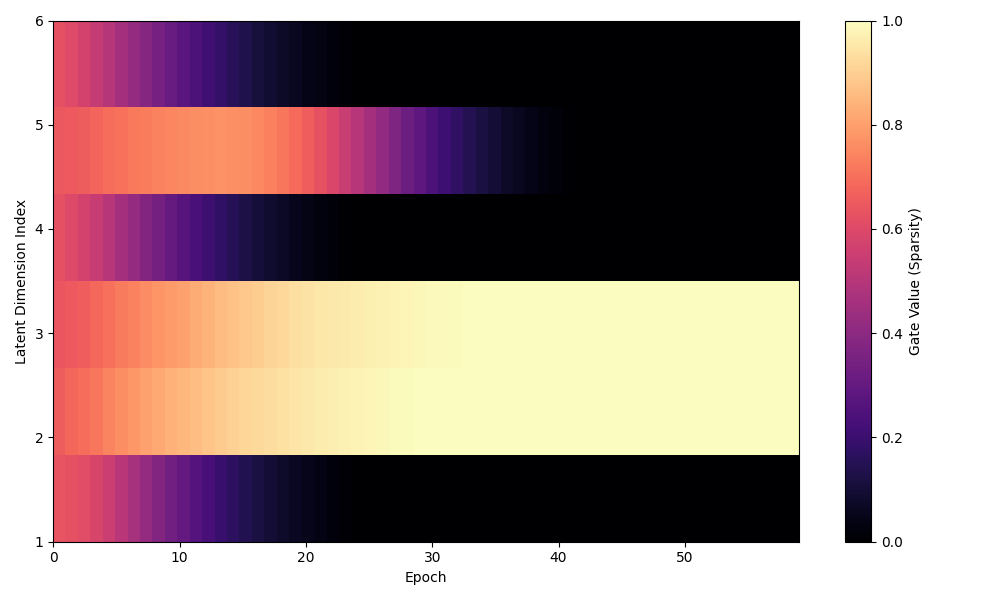
\includegraphics[width=\textwidth]{figures/numerical_indep_gate_history.png}
    \caption{Gate convergence history.}
  \end{subfigure}
  \hfill
  \begin{subfigure}[b]{0.48\textwidth}
    \centering
    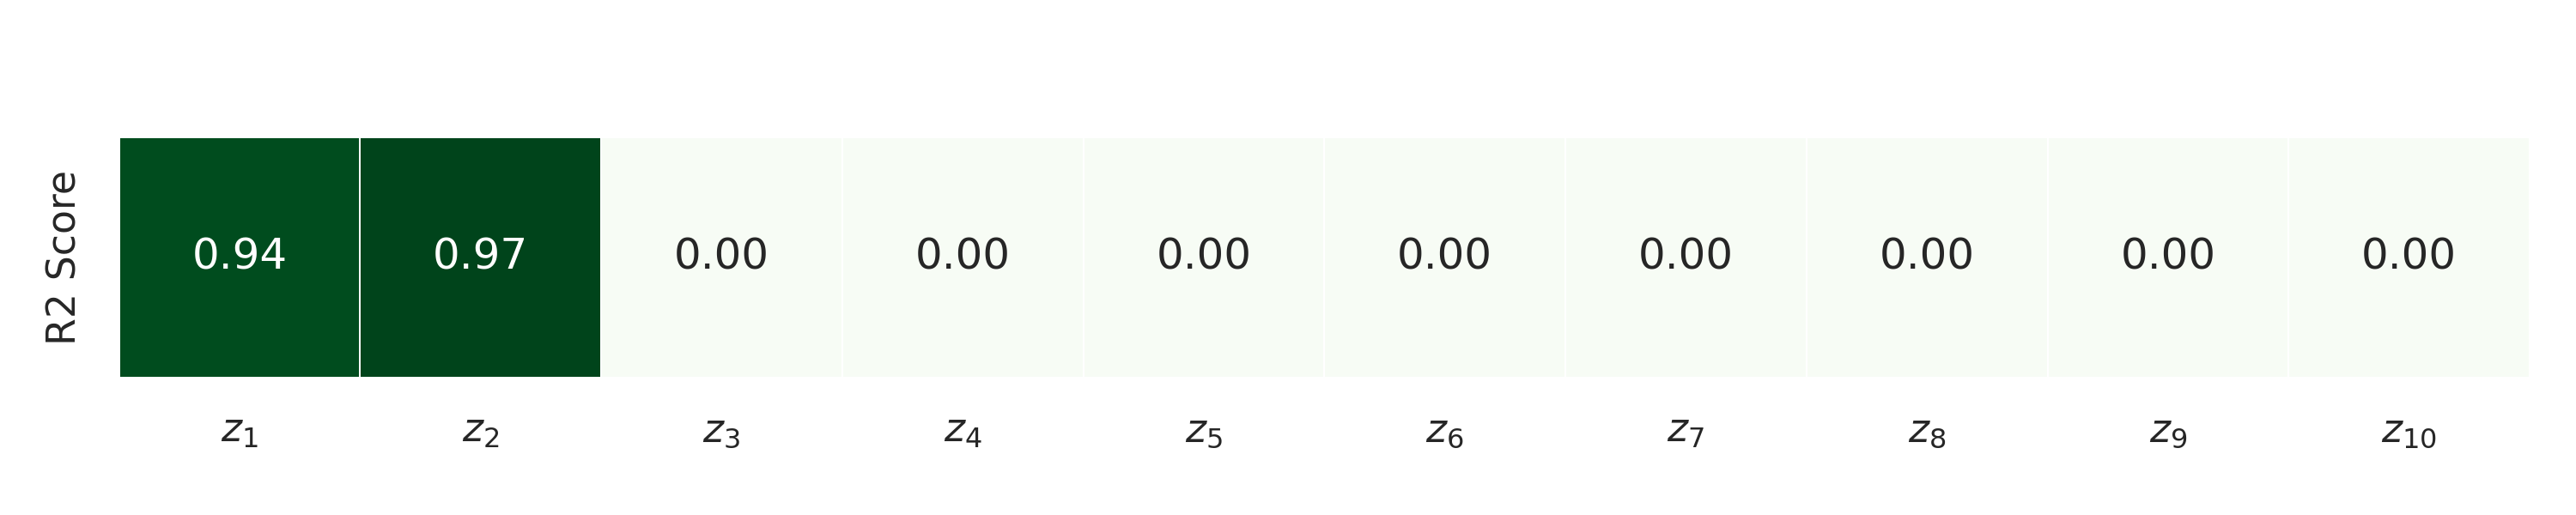
\includegraphics[width=\textwidth]{figures/numerical_indep_r2.png}
    \caption{$R^2$ scores per dimension.}
  \end{subfigure}
  \caption{\small{Numerical experiment results: (a) convergence of the hard concrete gate across the six latent dimensions over the training duration. The gate maintains exactly two active dimensions in the end, which is consistent with the true number of content factors; (b) the $R^2$ scores show that the content factors are successfully block-identified, whereas style factors are ignored.}}
  \label{fig:num_exp_indep}
\end{figure}

\subsection{Multimodal Experiment}

We evaluate our approach on the Multimodal3DIdent dataset \cite{daunhawer2023identifiabilityresultsmultimodalcontrastive}, which pairs 3D image renderings (10 latent factors) with descriptive captions (5 latent factors). Crucially, only three factors---\texttt{object\_shape}, \texttt{object\_xpos}, and \texttt{object\_ypos}---are shared across modalities, constituting the global shared content $\mathbf{z}_{C}$ to be recovered.
Although both modalities include the \texttt{object\_color} latent, they are treated as style variables because they lack a bijective mapping; the image utilizes a continuous hue value, whereas the caption uses a discrete color name.
Our results are presented in Fig. \ref{fig:multi_exp}

Detailed latent specifications are provided in Appendix \ref{app:ExpDetails}, along with implementation details in Tab. \ref{tab:hyperparams_multi}.

\begin{figure}[H]
  \centering
  \begin{subfigure}[b]{0.48\textwidth}
    \centering
    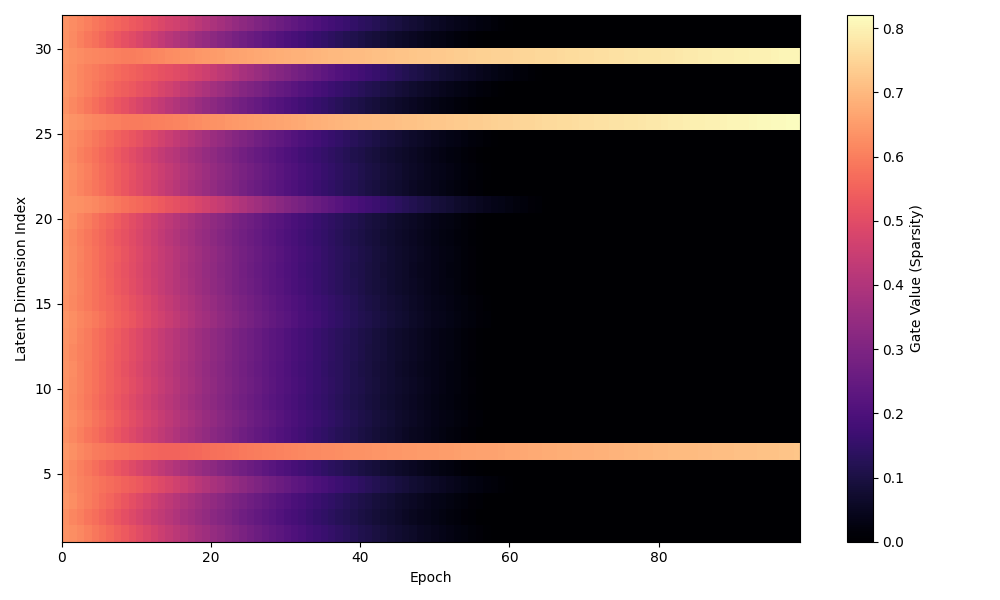
\includegraphics[width=\textwidth]{figures/multimodal_gate_history.png}
    \caption{Gate convergence history.}
  \end{subfigure}
  \hfill
  \begin{subfigure}[b]{0.48\textwidth}
    \centering
    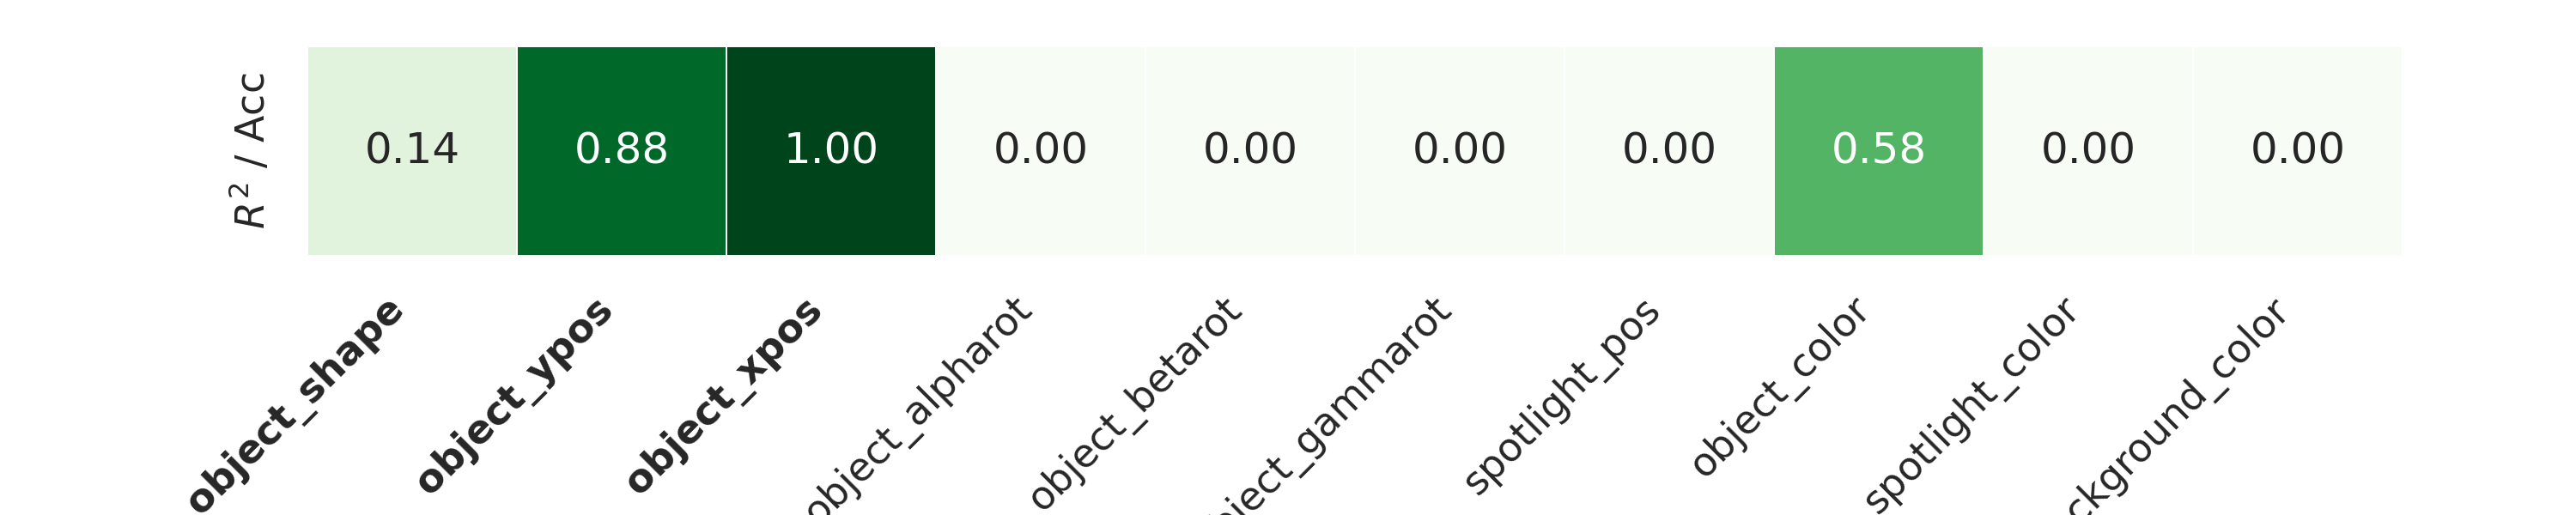
\includegraphics[width=\textwidth]{figures/multimodal_r2.png}
    \caption{Prediction performance per latent factor.}
  \end{subfigure}
  \caption{\small{Multimodal experiment results: (a) convergence of the hard concrete gate across 32 latent dimensions over the training duration; exactly three dimensions are kept active in the end, which is consistent with the true number of content factors. (b) the prediction performance is similar to \cite{daunhawer2023identifiabilityresultsmultimodalcontrastive}'s results; consistent with their findings, the recovery of the content \texttt{object\_shape} proved difficult, while the style \texttt{object\_color} factor achieved a high $R^2$ score due to the strong dependency between the different color latents specific to the image and text views.}}

  \label{fig:multi_exp}
\end{figure}

\section{Limitations and Future Work}
While our empirical results are strong, this work lacks formal proofs for the relaxed setting in which the only assumption is the overestimation of the content dimension.
Future research should establish the theoretical conditions required for block-identifiability under these assumptions.
Additionally, the impact of the degree of overestimation on recovery accuracy and training cost remains to be explored. Investigating the consequences of underestimation would also be an avenue of practical relevance for our approach.

\section{Conclusion}
In this work, we addressed the challenge of bridging the gap between theoretical identifiability and practical implementation in multi-view representation learning. Specifically, we introduced a differentiable shared masking mechanism that relaxes the restrictive requirement for prior knowledge of the latent space's exact dimensionality. By allowing for an overestimation of the content dimension, our approach provides a more robust and realistic framework for recovering global shared content. Empirical evaluations demonstrate that our method achieves performance comparable to previous works \cite{daunhawer2023identifiabilityresultsmultimodalcontrastive, yao2024multiviewcausalrepresentationlearning} that rely on oracle knowledge of latent dimensionality.

\newpage
\section*{Self-Assessment}

We feel quite satisfied with the outcome of the project, as we have not only addressed an important limitation of the existing literature (i.e., the assumption of known content dimension), but also proposed a practical solution that is both computationally efficient and elegant in identifying the global content. Given a second iteration, we would like to investigate the theoretical properties of our method to understand why it works so well in practice.

\section*{Statement on the Use of LLMs}

LLMs were used mostly for the coding portion of the project - partly to understand pre-written codebases from Yao and Daunhawer, and partly to assist in the implementation of our methods. They were also used in the writing portion to accelerate the drafting/formatting of the report (which was then thoroughly edited by us).
LLMs were also used as a research tool to aid in finding and understanding relevant literature.

\section*{Statement on Contributions}

David wrote the majority of the code for the model architectures and designed the numerical experiment.
He also handled the writing about the experiment implementations and results and contributed significantly to the editing of the report.
Ryan wrote and edited the majority of the report and established most of the code for the multimodal experiment. David, Ryan, and Dowoo all contributed to preparing the final presentation.

\section*{Acknowledgements}

We would like to thank our professor, Dr. Siamak Ravanbakhsh, for his invaluable guidance and support throughout this project. We also give special thanks to Sébastien Lachapelle for his insightful feedback and suggestions that steered us in the right direction.

\newpage
\bibliographystyle{unsrt}
\bibliography{ref.bib}

\newpage
\appendix
\begin{center}
  \Huge \textbf{Appendix}
\end{center}

\section{Definitions for Section \ref{sec:theory}} \label{app:definitions}

\begin{definition}[Block-Identifiability]
  \label{def:block_id}
  The true content variables $\mathbf{c}$ are block-identified by a function $g: \mathcal{X} \rightarrow \mathbb{R}^{\text{dim}(\mathbf{c})}$ if the inferred content partition $\hat{\mathbf{c}} = g(\mathbf{x})$ contains all and only information about $\mathbf{c}$. That is, there exists some smooth invertible mapping $h$ such that $\hat{\mathbf{c}} = h(\mathbf{c})$.

  In essence, block-identifiability ensures that the learned representation captures the shared content variables without including any extraneous information from the style variables.
\end{definition}

\begin{definition}[Selection Operator]
  For a binary mask $\mathbf{a} \in \{0, 1\}^d$ and a vector $\mathbf{b} \in \mathbb{R}^d$, the operator $\oslash$ is defined as:
  $$\mathbf{a} \oslash \mathbf{b} := [\mathbf{b}_j : \mathbf{a}_j = 1, j \in [d]].$$
\end{definition}

\section{Theoretical Foundations} \label{app:theory}

Our approach is inspired by the identifiability results of Yao et al. \cite{yao2024multiviewcausalrepresentationlearning}, which we present below.
First, their theoretical guarantees require the following assumptions:
\begin{assumption}[General Assumptions] \label{genAsm}
  For the generative model defined in Section \ref{sec:theory}:
  (i) Each view-specific mixing function $f_k$ is a diffeomorphism;
  (ii) $p_\mathbf{z}$ is a smooth and continuous density with $p_\mathbf{z} > 0$ almost everywhere.
\end{assumption}

Now, we introduce some more general notation.
Let $\mathcal{V} := \{V \subseteq [K] : |V| \ge 2\}$ denote the collection of subsets $V \in \mathcal{V}$ indexing two or more views.
For $V \in \mathcal{V}$, we denote the subset of views as $x_V := \{x_k : k \in V\}$. The corresponding shared content indices are given by the intersection of the view-specific indexing sets:
\begin{equation*}
  C_V = \bigcap_{k \in V} S_k,
\end{equation*}
so that the associated content latent variables can be written as $\mathbf{z}_{C_V} := \{\mathbf{z}_j : j \in C_V\}$.

Their first guarantee states that for any fixed subset $V \in \mathcal{V}$, the shared content is block-identifiable using \textit{content encoders} $g_k$, which we define below.

\begin{definition}[Content Encoders]
  \label{def:content_enc}
  Assuming the content size $|C|$ is given for a set of jointly observed views $x_V$, the content encoders $G := \{g_k : \mathcal{X}_k \rightarrow (0, 1)^{|C|}\}_{k \in V}$ consist of smooth functions mapping the respective observation spaces to the $|C|$-dimensional unit cube.
\end{definition}

\begin{theorem}[Block-identifiability from a Fixed Set of Views \cite{yao2024multiviewcausalrepresentationlearning}] \label{thm:contBlock}
  Under Asm.\ \ref{genAsm}, let $G = \{g_k\}_{k \in V}$ be a set of content encoders that minimizes:
  \begin{equation}
    \mathcal{L}(G) = \underbrace{\sum_{k < k' \in V} \mathbb{E} \left[ \|g_k(\mathbf{x}_k) - g_{k'}(\mathbf{x}_{k'})\|_2 \right]}_{\text{Content Alignment}} - \underbrace{\sum_{k \in V} H(g_k(\mathbf{x}_k))}_{\text{Entropy regularization}}
  \end{equation}
  where $H(\cdot)$ denotes differential entropy and the expectation is over $p(\mathbf{x}_V)$. Then $\mathbf{z}_{C_V}$ is block-identified by $g_k \in G$ for any $k \in V$.
\end{theorem}

Intuitively, the content alignment term encourages the content encoders to produce similar representations for the shared content across the views in $V$, while the entropy regularizer prevents the encoders from collapsing to trivial solutions (e.g., constant functions). However, this result requires training separate encoders for each subset of views, which is computationally infeasible as the number of subsets grows exponentially with the number of views.

Hence, to avoid the computational burden of retraining encoders for every subset, their subsequent result introduces learned \textit{content selectors} (masks) and \textit{projections} to achieve simultaneous block-identifiability across all $V \in \mathcal{V}$ using shared \textit{view-specific encoders}.

\begin{definition}[View-Specific Encoders]
  \label{def:view_enc}
  The view-specific encoders $R := \{r_k : \mathcal{X}_k \rightarrow \mathcal{Z}_{S_k}\}_{k \in V}$ consist of smooth functions mapping from the respective observation spaces to the view-specific latent space, where the dimension of the $k$-th latent space $|S_k|$ is assumed to be known.
\end{definition}

\begin{definition}[Content Selectors]
  \label{def:content_select}
  The content selectors $\Phi := \{\phi_V^k : V \in \mathcal{V}, k \in V\}$ are learnable binary vectors, with $\phi_V^k \in \{0, 1\}^{|S_k|}$, that perform element-wise selection on the encoded representation such that $\phi_V^k \oslash r_k(x_k)$ extracts the selected representation.
\end{definition}

\begin{definition}[Projections]
  \label{def:proj}
  The set of projections $T := \{t_k\}_{k \in V}$ consist of smooth functions $t_k : \mathcal{Z}_{S_k} \rightarrow (0, 1)^{|S_k|}$ mapping each view-specific latent space to a hyper unit-cube of the same dimension $|S_k|$. These enforce invertibility of the encoders without interfering with disentanglement.
\end{definition}

\begin{theorem}[Simultaneous Identifiability via Masking \cite{yao2024multiviewcausalrepresentationlearning}] \label{thm:allContBlocks}
  Under Asm.\ \ref{genAsm}, let view-specific encoders $R = \{r_k\}$, content selectors $\Phi = \{\phi_V^k\}$, and projections $T = \{t_k\}$ solve:
  \begin{equation}
    \min \text{Reg}(\Phi) := \sum_{V \in \mathcal{V}} \sum_{k \in V} \| \phi_V^{k} \|_0 \quad \text{subject to:} \quad R, \Phi, T \in \arg\min \mathcal{L}(R, \Phi, T)
  \end{equation}
  where $\text{Reg}(\Phi)$ is an $L_0$ sparsity penalty on the selectors, and the base loss is:
  \begin{equation}
    \mathcal{L}(R, \Phi, T) = \sum_{V \in \mathcal{V}} \sum_{k < k' \in V} \mathbb{E} \left[ \|\phi_V^k \oslash r_k(\mathbf{x}_k) - \phi_V^{k'} \oslash r_{k'}(\mathbf{x}_{k'})\|_2 \right] - \sum_{k \in V} H(t_k \circ r_k(\mathbf{x}_k))
  \end{equation}
  Then for any $V \in \mathcal{V}$ and $k \in V$, the masked representation $\phi_V^k \oslash r_k$ block-identifies $\mathbf{z}_{C_V}$.
\end{theorem}

The regularity term $\text{Reg}(\Phi)$ encourages the model to find a sparse selection of dimensions that are shared across the views in $V$, preventing trivial solutions where all dimensions are labeled as shared. The content encoders $R$ learn to extract representations from each view, while the selectors $\Phi$ determine which dimensions correspond to the shared content for each subset of views. The projections $T$ further ensure that the representations have sufficient entropy to avoid collapse.

\section{Detailed Approach and Formulations} \label{app:approach_details}

\subsection{Hard Concrete Masking}
The discrete $L_0$ penalty is non-differentiable. Following \cite{louizos2018learningsparseneuralnetworks}, we treat each entry of the shared mask $\phi_j$ as a stochastic gate sampled from a Bernoulli distribution. To enable gradient-based optimization, we use the hard concrete distribution to ``stretch'' a continuous variable $s$ into the interval $(\gamma, \zeta)$, where $\gamma < 0$ and $\zeta > 1$. The mask $\tilde{\phi}_j$ is obtained via a hard-sigmoid:
\begin{equation}
  s = \text{Sigmoid} \left( \frac{\log u - \log(1-u) + \log \alpha_j}{\beta} \right), \quad \tilde{\phi}_j = \min(1, \max(0, s(\zeta - \gamma) + \gamma))
\end{equation}
where $u \sim \mathcal{U}(0,1)$, $\log \alpha_j$ is the location parameter, and $\beta$ is the temperature. This allows the information-sharing regularizer $\text{Reg}(\phi)$ to be implemented as a fully differentiable complexity loss:
\begin{equation}
  \text{Reg}(\phi) = \sum_{j=1}^d \text{Sigmoid}\left(\log \alpha_j - \beta \log \frac{-\gamma}{\zeta}\right).
\end{equation}
At test time, we obtain deterministic masks using the expected estimator:
\begin{equation}
  \hat{\phi}_j = \min(1, \max(0, \text{Sigmoid}(\log \alpha_j)(\zeta - \gamma) + \gamma)).
\end{equation}

\subsection{Multiview Symmetric InfoNCE}
Let $\hat{\mathbf{z}}_k = \tilde{\phi} \oslash r_k(\mathbf{x_k})$ be the masked representation for view $k$. To ensure joint alignment across all $K$ views, we employ a Symmetric InfoNCE loss \cite{oord2019representationlearningcontrastivepredictive, radford2021learning}, aggregated across all unique pairs $(k, k')$:
\begin{equation}
  \mathcal{L}_{\text{SymInfoNCE}} = \frac{1}{K(K-1)B} \sum_{k=1}^K \sum_{k' \neq k} \sum_{i=1}^B -\log \frac{e^{\text{sim}(\hat{z}_{i,k}, \hat{z}_{i,k'})/\tau}}{\sum_{j=1}^B e^{\text{sim}(\hat{z}_{i,k}, \hat{z}_{j,k'})/\tau}}
\end{equation}
where $B$ is the batch size, $\text{sim}(\cdot, \cdot)$ denotes the similarity measure (e.g., negative Euclidean distance or cosine similarity) and $\tau$ is the temperature parameter. The denominator acts as a surrogate for entropy maximization by contrasting paired representations against batch distractors, preventing the trivial solution of dimensional collapse.

\section{Experiments} \label{app:Exp}

\subsection{Experimental Details} \label{app:ExpDetails}

\paragraph{Multimodal Experiment with Multimodal3DIdent} The Multimodal3DIdent dataset \cite{daunhawer2023identifiabilityresultsmultimodalcontrastive} consists of $224 \times 224 \times 3$ RGB images paired with descriptive natural language captions. The images are rendered in Blender using 10 underlying factors: object shape (7 classes), x and y positions (3 discrete values each), 3D rotations (3 continuous angles), object color, spotlight position, spotlight color, and background color. The corresponding text is generated from 5 factors: shape, x-position, y-position, color names selected from random palettes, and one of five unique sentence templates that determine the phrasing style. Examples of the dataset are displayed in Fig. \ref{fig:multi_example}

\begin{figure}[htbp]
  \centering
  \centering
  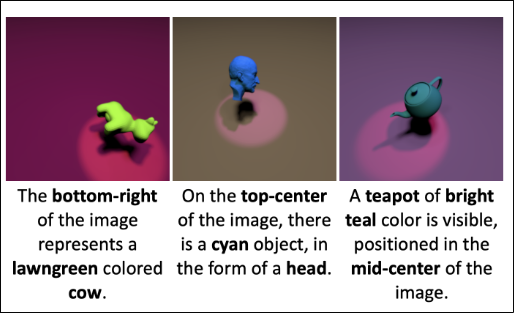
\includegraphics[width=0.6\textwidth]{figures/multi_example.png}
  \caption{Multimodal3DIdent Dataset - examples of image-caption pairs. Source: \cite{daunhawer2023identifiabilityresultsmultimodalcontrastive}}
  \label{fig:multi_example}
\end{figure}

The generative process is designed so that only three factors—object shape, x-position, and y-position—are identical across both modalities. While both views reference the object's color, the image uses continuous hue values while the text uses discrete names from varying palettes, preventing a direct one-to-one correspondence. All other factors, such as camera rotation, lighting, and sentence structure, are modality-specific.

\subsection{Implementation Details}
\label{app:implement_details}

In Tab. \ref{tab:hyperparams}, we lay out the model architectures and hyperparameters used for both the numerical and multimodal studies.
\begin{table}[ht]
  \centering
  \renewcommand{\arraystretch}{0.90}
  \begin{subtable}[t]{0.48\textwidth}
    \centering
    \small
    \begin{tabular}{@{}lr@{}}
      \toprule
      \textbf{Parameter} & \textbf{Value} \\ \midrule
      Generating function & 2-layer invertible MLP \\
      Encoder & 2-layer MLP \\
      Output dim. $d$ & 6 \\
      Optimizer & Adam \\
      Cond. threshold ratio & 1e-3 \\
      Batch size & 4096 \\
      Learning rate & 1e-3 \\
      Temperature $\tau$ & 2.0 \\
      \# Iterations & 6,000 \\
      Similarity metric & Cosine similarity \\ \bottomrule
    \end{tabular}
    \caption{Numerical simulation.}
    \label{tab:hyperparams_num}
  \end{subtable}
  \hfill
  \begin{subtable}[t]{0.48\textwidth}
    \centering
    \small
    \begin{tabular}{@{}lr@{}}
      \toprule
      \textbf{Parameter} & \textbf{Value} \\ \midrule
      Generating function & Image and text rendering \\
      Image encoder & ResNet-18 \\
      Text encoder & 4-layer ConvNet \\
      Output dim. $d$ & 32 \\
      Optimizer & Adam \\
      Batch size & 256 \\
      Learning rate & 1e-4 \\
      Temperature $\tau$ & 2.0 \\
      \# Iterations & 50,000 \\
      \# Samples (train/val/test) & 125k/10k/10k \\
      Similarity metric & Cosine similarity \\ \bottomrule
    \end{tabular}
    \caption{\textit{Multimodal3DIdent}.}
    \label{tab:hyperparams_multi}
  \end{subtable}
  \caption{Experiment Hyperparameters. Note that our experiments only use a fraction of the number of iterations used in \cite{yao2024multiviewcausalrepresentationlearning} and \cite{daunhawer2023identifiabilityresultsmultimodalcontrastive}, for computational efficiency, though the results remain competitive enough for comparison.}
  \label{tab:hyperparams}
\end{table}

\subsection{Additional Numerical Experiment Results} \label{app:AdditonalExpResults}
We remodel the numerical study to allow for \textit{causally dependent} latent factors $\mathbf{z} \sim \Normal(0, \mathbf{\Sigma}_{\mathbf{z}})$ via a non-trivial covariance matrix $\Sigma_\mathbf{z} \sim \mathrm{Wishart}(0, \mathbf{I}_\mathbf{z})$. Even under this formulation, Fig. \ref{fig:num_exp_dep} shows that the content factors are block-identified using the correct number of dimensions. This shows that our method is also robust to causal dependencies between the latent variables, which is a common scenario in real-world applications.

\begin{figure}[htbp]
  \centering
  \begin{subfigure}[b]{0.48\textwidth}
    \centering
    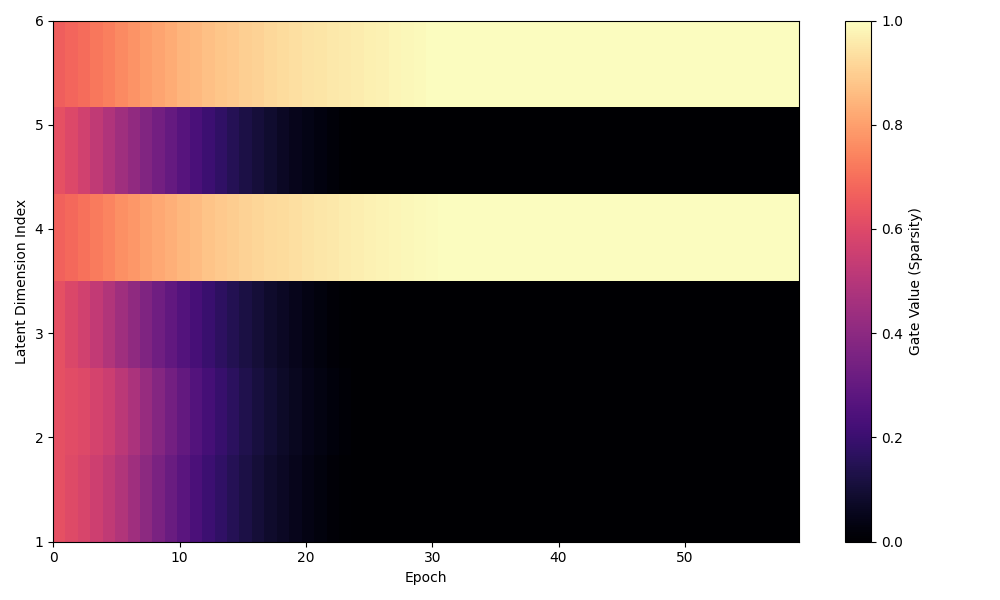
\includegraphics[width=\textwidth]{figures/numerical_dep_gate_history.png}
    \caption{Gate convergence history.}
  \end{subfigure}
  \hfill
  \begin{subfigure}[b]{0.48\textwidth}
    \centering
    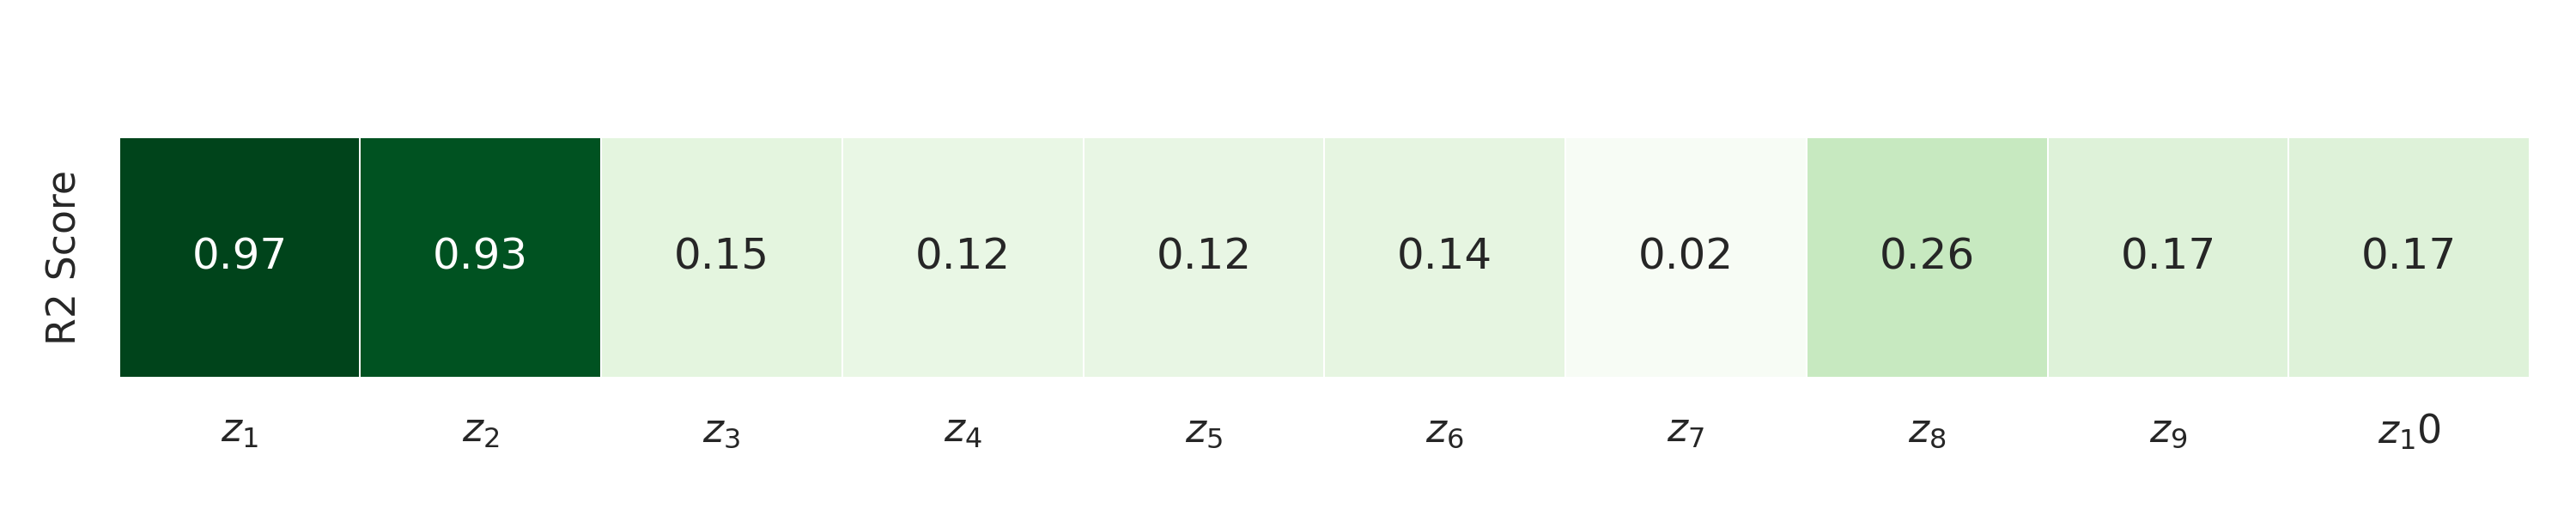
\includegraphics[width=\textwidth]{figures/numerical_dep_r2.png}
    \caption{$R^2$ scores per latent factor.}
    \label{fig:num_exp_dep_r2}
  \end{subfigure}
  \caption{Numerical experiment with dependent factors: (a) even in the case where the latent factors are causally dependent, the model still learns the correct number of content dimensions - (b) the $R^2$ scores also indicate that block-identifiably has been achieved, and the style factors now have non-zero $R^2$ values due to the latent dependencies.}
  \label{fig:num_exp_dep}
\end{figure}

\end{document}
